\documentclass{standalone}

\usepackage{tikz}
\usetikzlibrary{positioning}
\usetikzlibrary{calc}


\begin{document}

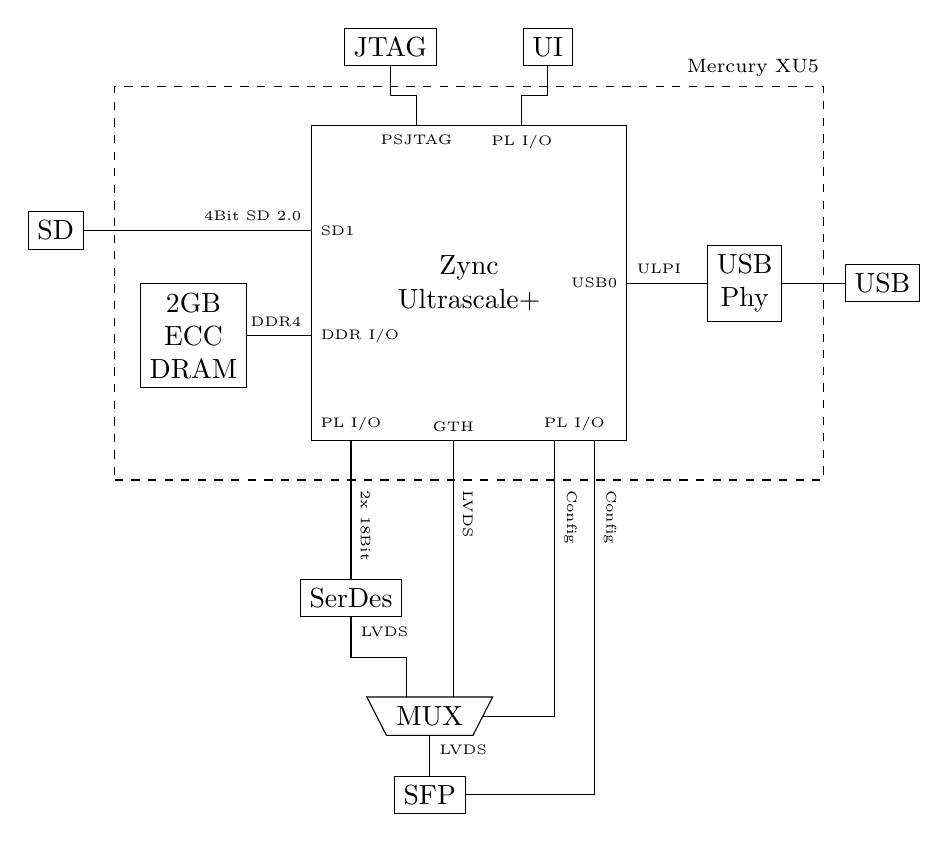
\begin{tikzpicture}
    %\draw[step=1cm,gray,very thin] (-4.9,-4.9) grid (4.9,4.9);
    %Soc
    \node[draw, minimum height=4cm, minimum width=4cm, align=center] (soc) at (0,0) {Zync\\Ultrascale+};
    %XU5
    \node[draw, dashed, minimum height=5cm, minimum width=9cm, align=center] (xu) at (0,0) {};
    \node[anchor=south] at ($(xu.north west)!9/10!(xu.north east)$) {\scriptsize Mercury XU5};
    %JTAG
    \node[draw] at (-1,3) (jtag) {JTAG};
    %UI
    \node[draw] at (1,3) (ui) {UI};
    %SD
    \node[draw] at ({-5.25,0} |- {$(soc.north west)!1/3!(soc.south west)$}) (sd) {SD};
    %DRAM
    \node[draw, align=center] at ({-3.5,0} |- {$(soc.north west)!2/3!(soc.south west)$}) (dram) {2GB\\ECC\\DRAM};
    %SerDes
    \node[draw] at (-1.5, -4) (serdes) {SerDes};
    %MUX
    \def\xmux {.25cm} %MUX amount of longer input sides
    \node at (-0.5,-5.5) (mux) {MUX};
    \draw (mux.south west) -- (mux.south east) -- ([xshift=\xmux]mux.north east) -- ([xshift=-\xmux]mux.north west) -- (mux.south west);
    %SFP
    \node[draw] at (-0.5,-6.5) (sfp) {SFP};
    %USB Phy
    \node[draw, align=center] at (3.5,0) (usbPhy) {USB\\Phy};
    %USB
    \node[draw] at (5.25,0) (usb) {USB};

    %FPGA - JTAG
    \draw ($(soc.north west)!1/3!(soc.north east)$) |- ({jtag} |- {$(soc.north)!0.5!(jtag.south)$}) node[pos=0, anchor=north] {\tiny PSJTAG} -- (jtag) ;
    %FPGA - UI
    \draw ($(soc.north west)!2/3!(soc.north east)$) |- ({ui} |- {$(soc.north)!0.5!(ui.south)$}) node[pos=0, below] {\tiny PL I/O} -- (ui) ;
    %FPGA - SD
    \draw ($(soc.north west)!1/3!(soc.south west)$) -- (sd) node[pos=0.0, sloped, anchor=south east] { \tiny 4Bit SD 2.0} node[pos=0, anchor=west] {\tiny SD1};
    %FPGA - DRAM
    \draw ($(soc.north west)!2/3!(soc.south west)$) -- (dram) node[pos=0, anchor=south east] {\tiny DDR4} node[pos=0, anchor=west] {\tiny DDR I/O};
    %FPGA - SerDes
    \draw (soc.south -| serdes) -- (serdes) node[yshift=-0.5cm, pos=0, anchor=south west, rotate=-90] {\tiny 2x 18Bit} node[pos=0, above] {\tiny PL I/O};

    \def\xi{.25cm}; %xshift of Datainputs of MUX
    %SerDes - MUX
    \draw (serdes.south) |- ([xshift=\xi]{mux.north west} |- {$(mux.north west)!0.5!(serdes.south)$}) -- ([xshift=\xi]mux.north west);
    \node[anchor=north west] at (serdes.south) {\tiny LVDS};
    %FPGA - MUX DAtA
    \draw ([xshift=-\xi]mux.north east) -- ([xshift=-\xi]soc.south -| mux.north east) node[yshift=-0.5cm, pos=1, anchor=south west, rotate=-90] {\tiny LVDS} node[pos=1, anchor=south] {\tiny GTH};
    %FPGA - MUX Config
    \draw ([xshift=\xmux/2]mux.east) -| ([xshift=-0.25cm]$(soc.south)!2/3!(soc.south east)$) node[anchor=south west, rotate=-90, xshift=0.5cm] {\tiny Config}; 
    %MUX - SFP
    \draw (mux) -- (sfp) node[pos=0, anchor=north west] {\tiny LVDS}; 
    %FPGA - SFP
    \draw (sfp.east) -| ([xshift=0.25cm]$(soc.south)!2/3!(soc.south east)$) node[anchor=south west, rotate=-90, xshift=0.5cm] {\tiny Config};
     \node[above] at ($(soc.south)!2/3!(soc.south east)$) {\tiny PL I/O};
    %FPGA - USB PHY
    \draw (usbPhy) -- (soc) node[pos=1, anchor=south west] {\tiny ULPI} node[pos=1, anchor=east] {\tiny USB0};
    %USB Phy - USB
    \draw (usbPhy) -- (usb);

    
\end{tikzpicture}

\end{document}